% Merged two-game metagame-prediction paper.
% Study 1 (Pokemon) condensed from post_sub/metagame_pipeline/paper/main.tex.
% Study 2 (Hearthstone) condensed from
%   phd/hearth-mici/papers/metagame_prediction/main.tex (3-seed / pair-bias /
%   mass-match pipeline, de-claude pass 2026-08-15).
% New material: Introduction, "A Common Problem" (Sec III), Cross-Game
% Synthesis (Sec VI). Both source papers are kept intact for comparison.
% All numbers copied from the two source drafts' committed artifacts.
% Bibliography merged and de-duplicated in refs.bib.
% Figure palette (Hearthstone plots): blue #2A78D6 measured, orange #EB6834
% model, gray context; CVD-safe, >=3:1 print contrast.
% Venue: IEEE Transactions on Games (journal).

\documentclass[journal]{IEEEtran}

\usepackage{cite}
\usepackage{amsmath}
\usepackage{booktabs}
\usepackage{url}
\usepackage{graphicx}
\usepackage{xcolor}
\usepackage{tikz}
\usetikzlibrary{positioning,arrows.meta,calc}
\usepackage{pgfplots}
\pgfplotsset{compat=1.18}

\definecolor{vizblue}{HTML}{2A78D6}
\definecolor{vizorange}{HTML}{EB6834}
\definecolor{vizgray}{HTML}{898781}
\definecolor{vizgrid}{HTML}{E1E0D9}
\definecolor{vizaxis}{HTML}{C3C2B7}
\definecolor{vizink}{HTML}{52514E}

\newcommand{\pp}{\,\text{pp}}
\newcommand{\pkmn}{Pok\'emon}

\begin{document}

\title{What Simulation Predicts About a Shifting Metagame:\\
A Study in \pkmn{} and Hearthstone}

\author{Alex Elton-Pym and Kazjon Grace%
\thanks{The authors are with The University of Sydney, Sydney, Australia
(e-mail: alex.elton-pym@sydney.edu.au; kazjon.grace@sydney.edu.au).}}

\markboth{Preprint}{}

\maketitle

\begin{abstract}
Balance patches and expansions shift a competitive game's metagame, the
mix of cards or species its players favor. We test what simulation
actually predicts about that shift, in two games with independent
pipelines: a replication of Saravanan and Guzdial's meta discovery
framework in \pkmn{} Showdown, extended from four hand-picked bans to 42
consecutive months of ordinary drift, and a marginal-value probe driving
evolutionary deckbuilding in Hearthstone, predicting card adoption across
the Naxxramas expansion and the Starving Buzzard nerf against 33{,}697
real decklists. The two studies agree: a no-change baseline is hard to
beat at naming the metagame's members, since most of a metagame is
stable; what simulation does predict is how much the metagame will move;
methods that feed on their own predictions degrade until grounded in
real data; and the real usage a pipeline starts from carries more
predictive content than the simulation on top of it. We contribute two
methods aimed at the movement signal and an evaluation standard for
future work on this task.
\end{abstract}

\begin{IEEEkeywords}
Metagame, game balance, replication, \pkmn{}, Hearthstone,
evolutionary computation.
\end{IEEEkeywords}

\section{Introduction}

\IEEEPARstart{D}{evelopers} of competitive multiplayer games adjust
balance continuously, and each adjustment can move the metagame, the set
of characters, cards, or strategies the player base currently favors.
Designers would like to anticipate that movement before a change goes
live, and a line of work on automated balancing evaluates proposed
changes inside a simulator. For most of its history that work scored its
predictions against a metagame internal to the simulator, with no check
against what a real player population went on to do. Saravanan and
Guzdial~\cite{saravanan2024framework} closed that gap for \pkmn{}
Showdown: their meta discovery framework builds teams from usage
statistics, plays them against each other with an automated agent, and
reads a predicted metagame off the resulting pick statistics, validated
against Smogon's measured post-ban usage for four historical bans, where
it recovered 92.5--100\% of the true post-ban meta.

Four hand-selected ban scenarios establish that the method can work.
They leave open how wide its operating envelope is, how it behaves when
the balance change is small or absent, and which part of the pipeline
carries the predictive content. A single-game
demonstration also leaves open whether any conclusion is a property of
metagame prediction or a property of \pkmn{}. We take up both questions
with two studies in two games, run as independent pipelines with
independent codebases and ground truth.

The first study stays in \pkmn{} Showdown and treats the original
framework directly. We reimplement its best configuration and evaluate it
on a completed \{generation\}$\times$\{rating cutoff\} grid: the four
original Generation~8 bans rerun at the full battle budget, and 42
consecutive monthly transitions of Generation~9 OverUsed (gen9ou), most
of which contain no balance change and therefore stress a method built
for balance changes. Monthly usage files are published on a fixed
schedule in a fixed format, so the drift regime supplies dozens of
objective test cases where the original had four.

The second study moves to Hearthstone, a collectible card game, and
builds a different pipeline for a different shock type. Where a ban
removes a legal option, an expansion adds new cards with no prior
usage (thirty, for Naxxramas) and a nerf leaves a card legal at a lower power level. We seed
evolutionary deckbuilding with the real pre-shock decks, played by
self-play-trained search agents on a purpose-built engine, and, because
whole-deck evaluation cannot resolve the value of a single card at
feasible budgets, we bias the search with a marginal-value probe that
measures each card's contribution in fixed real host decks. Ground truth
is 33{,}697 ranked 2014 decklists spanning the Naxxramas expansion and
the September 2014 Starving Buzzard nerf.

Read together, the two studies agree on more than either shows alone:

\begin{enumerate}
\item \emph{Composition is the wrong yardstick.} In both games a
no-change baseline wins the standard composition-overlap metric: \pkmn{}
no-change beats the framework on overlap in every cell of the grid, and
the Hearthstone no-change baseline ties or beats the pipeline on the
overall adoption rank correlation. Overlap saturates near its ceiling because most of a
metagame is stable month to month, so it measures stability more than
prediction.
\item \emph{Movement is the signal a simulator recovers.} What both
pipelines predict is how much the metagame moves. \pkmn{} self-play
matches the magnitude of monthly ranking change better than no-change
in 42 of 42 transitions at a high-ladder cutoff, and Hearthstone
probe-biased evolution predicts the direction and rough size of adoption
changes on the cards that actually moved, including the Buzzard collapse
from 73\% to a predicted 6\% against a real 17\%.
\item \emph{Self-referential usage loops fail the same way in both.} The
\pkmn{} framework's usage refresh feeds the team builder its own output,
and the Hearthstone free-running forecast feeds evolution its own
previous population as the evaluation field. Both drift from what players
did: battle outcomes do not enter the \pkmn{} usage update, while
Hearthstone's simulated selection does not prevent drift. In both,
grounding the method in real data improves the forecasts.
\item \emph{Use of simulated outcomes.}
The tested \pkmn{} ABC-Meta configuration builds teams from real usage
and base stats, then predicts usage by counting appearances on those
teams. Wins and losses do not affect the counts, so removing the battles
leaves the predictions almost unchanged. In Hearthstone, simulated games
measure the win-rate change from inserting a card into a real deck.
These measurements guide mutation, and further games determine which
evolved decks survive. Unguided evolution did not reliably find the
relevant card improvements at the budgets tested. Our \pkmn{} surrogate
learns to estimate matchup win probabilities from simulated games and
uses those estimates to select teams. Its usage forecast is then blended
with the previous month's observed usage.
\item \emph{Two methods that target movement.} For \pkmn{} we contribute
a fast learned stand-in for the battle simulator whose predictions, read out by blending back toward last month's meta, track how much the meta moves two to three times more closely than assuming no change, at about one-seventeenth of simulation's cost. For Hearthstone we contribute the
marginal-value probe and probe-biased evolution, piloted by self-play
agents under hidden information, with an ablation showing that the
information the pilots have changes which cards the search finds.
\end{enumerate}

We regard the \pkmn{} study as a friendly replication: the original
results reproduce on their own scenarios, and the cells where the
framework loses pair the original's data with regimes it never evaluated
or claimed. The Hearthstone study is a new pipeline that reaches
the same methodological conclusions by an independent route. None of these findings depends on the other game, so we can state them as properties of the task rather than of one title.

\section{Related Work}

Automated analysis of game balance spans several genres. Jaffe et
al.~\cite{jaffe2012evaluating} proposed estimating competitive balance
from repeated games between AI agents, Volz et al.~\cite{volz2016demonstrating}
balanced a card game on simulated play alone, and Toma\v{s}ev et
al.~\cite{tomasev2020assessing} used AlphaZero to evaluate alternative
chess rule sets. de Mesentier Silva et al.~\cite{silva2019evolving}
evolved balance changes to Hearthstone cards toward a target win rate,
and Hernandez et al.~\cite{hernandez2020metagame} balanced competitive
games by optimizing over a parameterized metagame graph; Kavanagh et
al.~\cite{kavanagh2021chained} map an evolving metagame across rule
configurations by model checking, for games small enough to enumerate,
and Pfau et al.~\cite{pfau2023replicants} balance by simulating agents
cloned from player behaviour. These search for a change. A second line
measures or predicts what players do after one, without simulating the
game: Yue et al.~\cite{yue2022gospel} predict which Dota~2 heroes the
next patch will change from match records, He et
al.~\cite{he2021heterogeneous} show that League of Legends patches affect
players unequally by skill, Lee and Ramler~\cite{lee2015champion,lee2017nonmeta}
track how champion usage follows content updates and find strategies that
beat the settled meta, Elbert et al.~\cite{elbert2023layers} measure
several layers of adaptation to CS:GO patches, Pedrassoli Chitayat et
al.~\cite{chitayat2023beyond} show that esports analytics models break at
each patch, Heo and Kim~\cite{heo2026switch} predict strategy switches in
Clash Royale, whose meta is reshaped by frequent balance updates, and Codsi
and Vetta~\cite{codsi2021metagames} fit a dynamic metagame model to real
Smash Bros.\ character selection. Saravanan and
Guzdial~\cite{saravanan2024framework} instead predict the player-base
response to a change by simulation and validate it against real usage;
their framework is the direct subject of our first study and the
methodological anchor of the second.

\pkmn{} Showdown~\cite{showdown} has been a testbed since the
Showdown AI competition~\cite{lee2017showdown}; Huang and
Lee~\cite{huang2019selfplay} trained self-play battlers for it, the
PokeAgent Challenge~\cite{karten2026pokeagent} now runs Showdown self-play
at scale, and the poke-env library~\cite{sahovic2019pokeenv} provides the
agent interface used in the original study and here.
Metamon~\cite{metamon} trains competitive Showdown agents at scale; we use
battles from Metamon-derived agents as training data for our surrogate.
The VGC AI competition frames \pkmn{} team building as a meta-game balance
problem~\cite{reis2021vgc,reis2025vgc}, and Reis et
al.~\cite{reis2024adversarial} pit team-building agents against a balancing
agent that rewrites \pkmn{} attributes toward a diversity target; that
line changes the game to balance its meta, where we hold the change fixed
and predict the response. Ramos and Soria~\cite{ramos2026nash} analyse the
\pkmn{} trading-card metagame against tournament usage through its Nash
equilibria. For Hearthstone, the
game has served as an AI testbed for a decade. Garc\'ia-S\'anchez et
al.~\cite{garcia2016evodeck} established evolutionary deckbuilding, Bhatt
et al.~\cite{bhatt2018exploring} explored the Hearthstone deck space with
it, Fontaine et al.~\cite{fontaine2019mapelites} mapped that space with
quality-diversity search, Zhang et al.~\cite{zhang2022surrogate} replaced
the simulator inside that search with a learned surrogate, and
Fran\c{c}a et al.~\cite{franca2024creativestone} evolve variants of real
decks around a retained core; Q-DeckRec~\cite{chen2018qdeckrec} builds a
deck against one named opponent by reinforcement learning. Closest to our
card probe, Chen and Guy~\cite{chen2020chaos} score generated cards inside
an evolved meta and find that a card's strength depends on the meta it is
scored against, and Long et al.~\cite{long2023pointcosts} predict the
point cost a wargame unit should carry from play. The Hearthstone AI
competition~\cite{dockhorn2019competition} drove play agents, including
MCTS with learned components~\cite{swiechowski2018}. Justesen et
al.~\cite{justesen2017} showed that in multi-action adversarial games the
effective unit of decision is the turn plan. Determinized search has a
long record in hidden-information card games~\cite{long2010pimc}, and
Dockhorn et al.~\cite{dockhorn2018prediction} found that a Hearthstone
search agent gains substantially from knowing the opponent's hand and that
predicting the hand recovers most of that gain; our agents play under
hidden information throughout, and Section~\ref{sec:hsinfo} measures
directly what visible hands would change. Community analytics, the Vicious Syndicate Data Reaper
reports~\cite{vicious_syndicate}, Smogon usage
statistics~\cite{smogonstats}, and the HearthPwn deck
archive~\cite{zenodo_dataset}, supply ground truth. Both studies draw on
common machinery: MAP-Elites~\cite{mouret2015illuminating} for search
and Deep
Sets~\cite{zaheer2017deepsets} for permutation-invariant team and deck
encodings.

\section{A Common Problem, in Three Questions}
\label{sec:common}

Both studies ask the same thing. A game's \emph{metagame} is the mix of
cards or species players actually run~\cite{kokkinakis2021metagaming,silva2019evolving},
which we summarise as a ranking by how often each is used. Let $A$ be that ranking just before a rules change
(the pre-shock metagame), $B$ the ranking just after (the post-shock
metagame), and $B'$ a method's prediction of $B$ from $A$ and the rules
change alone. We judge $B'$ by three questions.

\begin{itemize}
\item \textbf{Which units?} Did $B'$ name the right cards or species, the
ones that make up the bulk of the meta? We call this \emph{composition}:
overlap of the top-$k$ lists of $B$ and $B'$ for \pkmn{}, and a rank
correlation between $B'$ and $B$ over all cards for Hearthstone.
\item \textbf{How much did it move?} A meta drifts a little most months and
lurches after a big change. Did $B'$ move about as far from $A$ as $B$ really
did, rather than sitting still or overshooting? We call this
\emph{movement}: for \pkmn{}, the edit-distance gap $|ED(A,B)-ED(A,B')|$,
where $ED$ is the mean rank shift over shared units; for Hearthstone, the
average error in predicted adoption.
\item \textbf{Which way?} Of the units that genuinely moved, did $B'$ call
the rises and falls correctly? We call this \emph{direction}: the fraction
of real movers whose direction it got right; for \pkmn{} we also report
Spearman's $\rho$ between the real rank changes $A{\to}B$ and the predicted
$A{\to}B'$.
\end{itemize}

Every method is measured against the same dumb yardstick: \emph{no change},
the guess $B'=A$ (the naive forecast of the forecasting
literature~\cite{hyndman2021fpp3}), with a banned unit removed where a ban
applies. No change is deceptively hard to beat on the
first question and trivial to beat on the third. Most of a meta is stable
across a change, so copying this month forward already names most of next
month's units, and a method that perturbs the meta can only lose ground
there. But no change predicts that nothing moves, so it is wrong on every
mover and scores zero on the third question by definition. A prediction earns
its keep on the second and third questions, how much the meta moves and which
way, not on the stable bulk the first rewards.

\section{Study 1: \pkmn{} Showdown}
\label{sec:pkmn}

\subsection{The Original Framework}

The framework~\cite{saravanan2024framework} has a battle agent, a team
builder, and a simulation environment that runs battles and compiles pick
statistics. Its ABC-Meta task assumes the true pre-change metagame and
builds six-species teams sequentially, scoring each species by
\begin{equation}
\mathrm{Score}_{\mathrm{ABC}}(x) = \mathrm{Pickrate}(x) \times \mathrm{BST}(x),
\label{eq:score}
\end{equation}
where $\mathrm{Pickrate}(x)$ is the fraction of team slots holding species
$x$ in current usage and $\mathrm{BST}(x)$ its normalized base stat total,
a form selected by a grid search over candidate components. Selection is
$\epsilon$-greedy ($\epsilon=0.001$), movesets come from Smogon's
per-species statistics, and the environment simulates 450{,}000 battles
per scenario, regenerating teams and refreshing the tracked usage every
1{,}000 battles. The predicted metagame is the top-40 species by resulting
pickrate. On four Generation~8 single-ban scenarios (OU, UU, NU, PU) the
method reached overlap 0.925--1.000 against a ban-aware naive baseline's
0.925--0.975, an edge of one species in three scenarios and a tie in the
fourth; edit-distance delta 0.11--2.74 against 3.04--6.84; and Spearman's
$\rho$ from $-0.15$ to $0.19$, never significant. The authors state that
their discovered meta reproduces composition and amount of change but not
the specific movement, and that the naive baseline has high overlap. Both
caveats organize what follows.

\subsection{Method}

We reimplemented the ABC-Meta pipeline from the paper's description,
using poke-env and \pkmn{} Showdown as the original did.
Figure~\ref{fig:pipelines} shows the three pipelines we compare. The team
builder draws species by \eqref{eq:score} from the input month's real
usage, samples a full set per species from that month's moveset
statistics, and validates every team with the @pkmn/sim
validator~\cite{pkmnps}. For each transition we generate two pools of 300
valid teams and play 10{,}000 self-play battles between two
\texttt{SimpleHeuristicsPlayer} instances on a local server, reading
predicted pickrate off appearances in finished battles. The exact-scenario
rerun (Section~\ref{sec:gen8}) instead uses the full 450{,}000-battle
budget, the refresh schedule, the banned species removed from the pool,
and the Little Cup blanket ban, matching the original.

The drift evaluation deviates from the original in ways we record so
readers can attribute each result: 10{,}000 battles rather than 450{,}000;
frozen month-$M$ statistics in the headline arm, with a faithful
refreshing variant in Section~\ref{sec:refresh}; the heuristic agent only,
which the original found statistically indistinguishable from its RL
agent; single-month Generation~9 transitions rather than three-month
Generation~8 ban windows; both rating cutoffs, the high-ladder 1695 files
and the unfiltered all-ratings files that Section~\ref{sec:gen8} ties to
the original's own data; and top-20 lists in the drift arm, where a
40-species list would cover most of the smaller monthly universe. The
gen8 rerun removes every deviation but the agent choice.

\begin{figure*}[t]
\centering
\resizebox{\textwidth}{!}{%
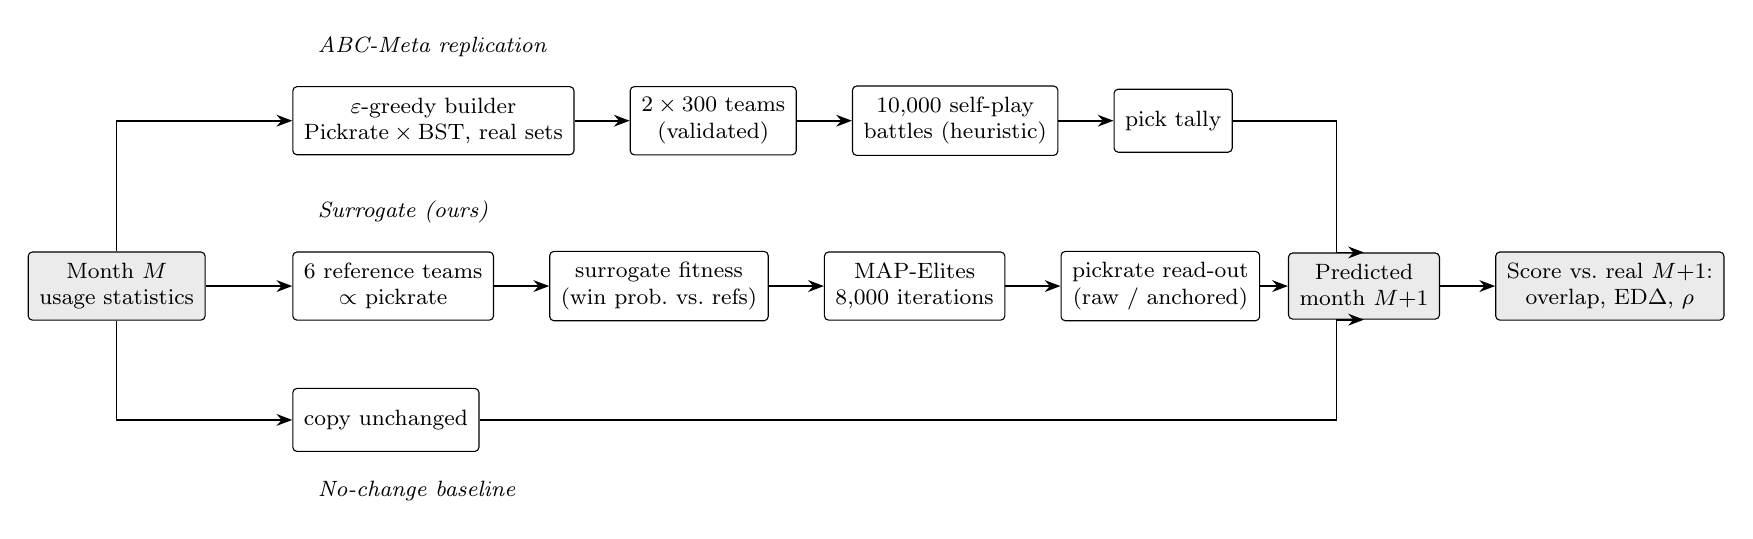
\begin{tikzpicture}[
  font=\footnotesize,
  box/.style={draw, rounded corners=1.5pt, align=center, inner sep=4pt, minimum height=8mm},
  io/.style={box, fill=black!8},
  arr/.style={-{Stealth[length=2mm]}, semithick},
  node distance=4mm and 7mm]
\node[io] (input) {Month $M$\\usage statistics};
\node[box, right=11mm of input, yshift=21mm] (builder) {$\varepsilon$-greedy builder\\$\text{Pickrate}\times\text{BST}$, real sets};
\node[box, right=of builder] (pools) {$2\times300$ teams\\(validated)};
\node[box, right=of pools] (battles) {10{,}000 self-play\\battles (heuristic)};
\node[box, right=of battles] (tally) {pick tally};
\node[box, right=11mm of input] (refs) {6 reference teams\\$\propto$ pickrate};
\node[box, right=of refs] (surr) {surrogate fitness\\(win prob.\ vs.\ refs)};
\node[box, right=of surr] (me) {MAP-Elites\\8{,}000 iterations};
\node[box, right=of me] (incl) {pickrate read-out\\(raw / anchored)};
\node[box, right=11mm of input, yshift=-17mm] (copy) {copy unchanged};
\node[io, right=of tally, yshift=-21mm] (pred) {Predicted\\month $M{+}1$};
\node[io, right=of pred] (score) {Score vs.\ real $M{+}1$:\\overlap, ED$\Delta$, $\rho$};
\draw[arr] (input) |- (builder);
\draw[arr] (builder) -- (pools);
\draw[arr] (pools) -- (battles);
\draw[arr] (battles) -- (tally);
\draw[arr] (input) -- (refs);
\draw[arr] (refs) -- (surr);
\draw[arr] (surr) -- (me);
\draw[arr] (me) -- (incl);
\draw[arr] (input) |- (copy);
\draw[arr] (tally) -| ([xshift=-3.5mm]pred.north) -- (pred.north);
\draw[arr] (incl) -- (pred);
\draw[arr] (copy) -| ([xshift=-3.5mm]pred.south) -- (pred.south);
\draw[arr] (pred) -- (score);
\node[anchor=west, font=\footnotesize\itshape] at ([xshift=2mm, yshift=5mm]builder.north west) {ABC-Meta replication};
\node[anchor=west, font=\footnotesize\itshape] at ([xshift=2mm, yshift=5mm]refs.north west) {Surrogate (ours)};
\node[anchor=west, font=\footnotesize\itshape] at ([xshift=2mm, yshift=-5mm]copy.south west) {No-change baseline};
\end{tikzpicture}%
}
\caption{The three \pkmn{} prediction pipelines. All start from the same
real month-$M$ usage statistics and are scored against real month $M{+}1$
with the same three metrics.}
\label{fig:pipelines}
\end{figure*}

\subsection{Movement Magnitude by Rating Cutoff}
\label{sec:r0}

At the high-ladder cutoff the framework's strongest claim holds.
ABC-Meta's edit-distance delta averages 3.87 on the full roster against
no-change's 21.21 (Table~\ref{tab:main}), and it is closer to the true
drift magnitude in 42 of 42 transitions (Wilcoxon $p\approx4.5\times
10^{-13}$). Since no-change's delta is the drift itself, the simulation
reproduces roughly the right amount of ranking movement where predicting
none misses by the full drift. This survives a 45$\times$ smaller battle budget in a new generation, with no ban to anchor the change.

At the all-ratings cutoff, the one Section~\ref{sec:gen8} identifies as
the original's own data, the same comparison reverses. ABC-Meta's mean
delta is 24.09 against no-change's 14.54, closer in only 5 of 42
transitions ($p=1.9\times10^{-4}$). The mechanism is in the two
no-change rows of Table~\ref{tab:main}: the all-games meta drifts less
than the high-ladder meta on the same months (14.54 against 21.21 rank
positions), because casual players spread usage widely and shift slowly.
The simulated meta has the opposite character, because the team builder,
scoring each species by its usage times its stat total, piles onto a few
high-scoring species.
Aimed at the sharp high-ladder target it moves by about the right amount;
aimed at the flat all-games target the same output implies two to three
times the movement that occurs. Nothing here contradicts a published
number. The failing cell pairs the original's cutoff with a regime it
never evaluated.

\begin{table*}[t]
\caption{\pkmn{} main results over 42 monthly transitions (mean $\pm$ sd).}
\label{tab:main}
\centering
\begin{tabular}{@{}llccc@{}}
\toprule
Method & Universe & Overlap (top-20) & Edit-distance $\Delta$ & Spearman $\rho$ \\
\midrule
ABC-Meta (replication) & full roster & $0.833 \pm 0.119$ & $3.87 \pm 5.28$ & $0.025 \pm 0.108$ \\
ABC-Meta (replication) & in-vocab & $0.875 \pm 0.095$ & $1.84 \pm 2.21$ & $0.065 \pm 0.144$ \\
Surrogate, raw read-out (ours) & in-vocab & $0.293 \pm 0.069$ & $23.17 \pm 4.80$ & $0.078 \pm 0.117$ \\
No-change & full roster & $0.886 \pm 0.118$ & $21.21 \pm 5.13$ & undefined \\
No-change & in-vocab & $0.907 \pm 0.089$ & $5.00 \pm 2.23$ & undefined \\
\midrule
ABC-Meta (replication) & full roster, rating 0 & $0.815 \pm 0.117$ & $24.09 \pm 7.22$ & $0.019 \pm 0.106$ \\
No-change & full roster, rating 0 & $0.888 \pm 0.110$ & $14.54 \pm 9.60$ & undefined \\
\bottomrule
\end{tabular}
\par\vspace{3pt}
\begin{minipage}{\textwidth}\footnotesize
Overlap and $\rho$: higher is better; edit-distance delta: lower is better.
Unlabeled rows are scored against the 1695 high-ladder statistics; rating-0
rows are the all-ratings rerun of Section~\ref{sec:r0}. No-change has no
defined $\rho$, and its edit-distance delta equals the true drift magnitude
by construction.
\end{minipage}
\end{table*}

\subsection{Composition Results}

No-change reaches 0.886 mean top-20 overlap on the full roster and
0.907 in-vocabulary; ABC-Meta reaches 0.833 and 0.875, losing the paired
comparison 31--2 ($p=2.6\times10^{-6}$) and 25--3 ($p=6.7\times10^{-5}$).
When 17 or 18 of next month's top 20 are this month's, any predictor that
reproduces the current meta scores high overlap, and a simulation that
perturbs the meta can only lose ground unless its perturbations are
unusually well aimed. Overlap here sits near its ceiling for reasons
unrelated to prediction, so it measures metagame stability more than
predictor skill. This does not indicate an error in the original study,
whose ban scenarios forced real compositional change and gave overlap
something to detect. It means the overlap advantage is specific to that
setting and should not be expected in the routine months that make up the
large majority.

\subsection{The Battle-Free Ablation}
\label{sec:battlefree}

Three independent observations show that in the ABC-Meta configuration the
battles' outcomes have no path into the prediction. First,
\eqref{eq:score} contains no outcome term; the tracked pickrates are
updated only from the teams the builder generated, so a battle influences
the statistics only by finishing and contributing its teams to the
counts. Second, the original's own tables report identical overlap for its
RL and heuristic agents (GXE 42.4\% against 49.4\%) in all four scenarios,
which is what outcome-independence predicts. Third, the pipeline runs with
the simulator deleted: the same builder, refresh schedule, and 450 updates
with zero battles reproduce the full-budget predictions almost unchanged
(Table~\ref{tab:gen8}, No-battle columns), in minutes on one core. The
8--14 hours of simulation per scenario buy sampling precision over the
builder's output distribution and nothing else. BSD-Meta, the framework's
other task, does consume winrates through its score, so this concerns only
the ABC configuration, whose grid-search winner happened to exclude every
outcome-dependent term.

\subsection{The Usage-Refresh Ablation}
\label{sec:refresh}

Our headline arm freezes the month-$M$ statistics. Implementing the
original's refresh faithfully, recomputing tracked pickrates from
accumulated picks every 1{,}000 battles, costs accuracy: mean overlap
falls from 0.833 to 0.801 (paired 25--5, $p=0.0009$) and edit-distance
delta worsens from 3.87 to 5.82 ($p=5.0\times10^{-5}$). The original
authors described the mechanism themselves, warning that scoring on a
statistic the builder updates would create an ``undesirable feedback
loop''~\cite{saravanan2024framework} that concentrates picks. ABC-Meta
contains that loop: its score reads pickrates, its refresh rewrites
pickrates from the builder's own output, and no battle outcome enters to
correct it. Freezing the statistics removes an uncorrected positive
feedback, so the real month's data grounds the whole run. The refreshing
variant still beats no-change on movement in 42 of 42 transitions, so
the central result stands under both configurations; the refresh only
erodes the margin.

\subsection{The Surrogate Arm}
\label{sec:surrogate}

The replication's cost is dominated by simulation, so we ask how much
survives when a learned model replaces it, the surrogate-assisted search
of evolutionary computation~\cite{jin2002framework,zhang2022surrogate}. A
Deep Sets
encoder~\cite{zaheer2017deepsets} embeds each team as a permutation-invariant
set, and a skew-symmetric bilinear head scores a matchup so that
$P(\text{A beats B})=1-P(\text{B beats A})$ by construction. A 430-species
model trained on 120{,}000 heuristic self-play battles reaches held-out
strength correlation 0.740 and trains in under five minutes on a consumer
CPU. To predict a transition we run MAP-Elites~\cite{mouret2015illuminating}
for 8{,}000 iterations over a $12\times12$ archive of speed and bulk, with
fitness the surrogate's win probability against a reference field sampled
from month-$M$ usage.

The search leaves us with a pool of strong, varied teams, and turning that
pool into a predicted usage ranking is a modelling choice that makes or
breaks the result. The obvious way, counting how often each species shows up
among the strong teams, predicts far too much upheaval: it names the right
units only $0.29$ of the time against no change's $0.91$. What works is to
let the strong teams play each other out, keep the ones that survive that
internal competition, and then \emph{blend the result back toward last
month's meta} (the same no-change yardstick from Section~\ref{sec:common}).
The blend supplies the stable bulk; the model supplies the movement on top.
With its settings fixed on the first 21 months and tested on the other 21,
this read-out tracks how much the meta moves two to three times more closely
than no change, at about 45 seconds per month against the full simulation's
13 minutes, and it keeps that edge on the harder all-games data where the full
simulation loses. Two honest caveats. The winning read-out was chosen after
seeing early results, so a test on genuinely future months is still owed. And
a control that replaced the model's output with random noise, blended the
same way, did not reproduce the result, so the model is doing real work
rather than the blend alone; what it does not do is call which way individual
species move any better than anything else here.

\subsection{Replicating the Four Original Scenarios}
\label{sec:gen8}

To separate what fails to transfer from what fails to reproduce, we reran
the four Generation~8 bans at the full 450{,}000-battle budget with the
refresh schedule intact. The unfiltered all-ratings files closely
reproduce the paper's published naive baselines (identical top-40 overlap
in OU, UU, NU, one species apart in PU), and their appendix's pickrate-only
grid-search row sits on top of our all-ratings OU baseline, so we take the
all-ratings files as the original's data. Table~\ref{tab:gen8} reports the
rerun: overlap within one species of the paper in every tier, matching
outright in PU, and the sign of Spearman's $\rho$ matching in all four
scenarios, a nontrivial agreement given that the original found none
significant. The overlap edge over the naive baseline is one species in PU
and a tie elsewhere, mirroring the original's one-species-or-tie margins
and confirming that margins this small need paired tests over many cases.
At high-ladder cutoffs (bottom block) the framework never wins overlap and
still beats the baseline on movement in three tiers of four, matching the
drift arm's split, and the battle-free pipeline reproduces the live run at
both cutoffs.

\begin{table*}[t]
\caption{The four original \pkmn{} scenarios rerun at the full
450{,}000-battle budget, top-40 lists. Paper values are the heuristic-agent
columns of the original's Tables~II--IV; naive columns delete the banned
species from pre-ban usage. No-battle is the identical pipeline with the
simulator removed (Section~\ref{sec:battlefree}). Top block: the original's
all-ratings statistics. Bottom block (HL): high-ladder statistics (1695 for
OU, 1630 otherwise), where the original reports no values.}
\label{tab:gen8}
\centering
\begin{tabular}{@{}l ccccc ccccc ccc@{}}
\toprule
& \multicolumn{5}{c}{Overlap} & \multicolumn{5}{c}{Edit-distance $\Delta$} & \multicolumn{3}{c}{Spearman $\rho$} \\
\cmidrule(lr){2-6} \cmidrule(lr){7-11} \cmidrule(lr){12-14}
Scenario & Ours & No-batt. & Naive & Paper & P.\ naive & Ours & No-batt. & Naive & Paper & P.\ naive & Ours & No-batt. & Paper \\
\midrule
OU & 0.950 & 0.950 & 0.950 & 0.975 & 0.950 & 2.65 & 2.70 & 2.75 & 1.09 & 3.04 & $+0.06$ & $+0.06$ & $+0.18$ \\
UU & 0.975 & 0.975 & 0.975 & 1.000 & 0.975 & 3.38 & 3.43 & 4.82 & 1.50 & 4.60 & $-0.19$ & $-0.20$ & $-0.13$ \\
NU & 0.925 & 0.925 & 0.925 & 0.950 & 0.925 & 4.12 & 4.01 & 5.46 & 2.49 & 5.57 & $-0.27$ & $-0.13$ & $-0.07$ \\
PU & 0.925 & 0.950 & 0.900 & 0.925 & 0.925 & 1.36 & 1.87 & 5.06 & 0.11 & 6.84 & $+0.19$ & $+0.14$ & $+0.15$ \\
\midrule
OU (HL) & 0.900 & 0.900 & 0.900 & --- & --- & 3.64 & 3.64 & 3.64 & --- & --- & $+0.14$ & $+0.21$ & --- \\
UU (HL) & 0.925 & 0.925 & 0.950 & --- & --- & 4.16 & 4.00 & 5.39 & --- & --- & $+0.14$ & $+0.11$ & --- \\
NU (HL) & 0.825 & 0.825 & 0.825 & --- & --- & 5.19 & 4.83 & 6.27 & --- & --- & $-0.06$ & $-0.02$ & --- \\
PU (HL) & 0.900 & 0.900 & 0.900 & --- & --- & 3.80 & 3.60 & 7.44 & --- & --- & $-0.06$ & $-0.08$ & --- \\
\bottomrule
\end{tabular}
\end{table*}

\subsection{The \pkmn{} Grid}

Table~\ref{tab:grid} compresses the study. The framework never wins
composition in any cell; its best showing is a single species in one ban
scenario. Movement carries all of its value, and that value is
conditional: simulation tracks how much a concentrated or shocked meta
will move, and on flat all-games ordinary drift it loses even that.
Which way individual species move stays unpredicted everywhere. Of the
species whose real usage shifted by more than five points between adjacent
months, ABC-Meta called the direction, rise or fall, right about half the
time ($0.53$). No change is wrong on every mover by construction, so it sets
no bar here; direction is a question neither method answers.

\begin{table}[t]
\caption{The completed \pkmn{} \{generation\}$\times$\{cutoff\} grid. Each
cell asks whether the framework beat its no-change baseline per transition
or per scenario; ties are omitted from W--L counts.}
\label{tab:grid}
\centering
\begin{tabular}{@{}llll@{}}
\toprule
Cell & Trigger & Movement (ED $\Delta$) & Composition \\
\midrule
gen9, 1695 & drift & won 42--0 & lost 2--31 \\
gen9, all games & drift & lost 5--37 & lost 3--32 \\
gen8, all games & 4 bans & won 4/4 & 1 win, 3 ties \\
gen8, high ladder & 4 bans & won 3/4, 1 tie & 1 loss, 3 ties \\
\bottomrule
\end{tabular}
\end{table}

\section{Study 2: Hearthstone}
\label{sec:hs}

The second study asks the same question in a collectible card game, with an independent codebase and ground truth, where the shocks are an expansion and a nerf rather than a ban.

\subsection{Simulator Fidelity}
\label{sec:hsfidelity}

The simulator is a purpose-built engine for Hearthstone's 2014 Classic
era. It implements the full 2014 pool (382 collectible Classic cards and
the 30 Naxxramas cards) on the era's rules, and the 245 cards the three
classes in this study (Hunter, Mage, Warrior) can play are each covered
by behavioural tests. A patch hook applies the September 2014 balance
changes (Starving Buzzard 2-mana 2/1 to 5-mana 3/2; Leeroy Jenkins 4 to 5
mana), giving three balance states: the pre-expansion pool, the expansion
at launch, and the post-nerf pool.

Decks are piloted by a search agent. A policy and value network reads the
game as a set of entities (each minion, hand card, and secret is a token
attended over by a single attention layer) and guides PUCT
search~\cite{rosin2011episodecontext,silver2017alphagozero}, trained by
self-play~\cite{silver2018alphazero} separately for each balance state, so the post-nerf agent has learned to play the nerfed
cards. All experiments use 200 search iterations per move. The agents are
trained and run under hidden information: a pilot sees its own hand and
both boards, and never the opponent's hand. A matching set of agents
trained with both hands visible serves the ablation in
Section~\ref{sec:hsinfo}.

Against a community matchup matrix from roughly 90k tracked games in
the 2021 Classic format, which replays the 2014 card pool at its June
2014 balance~\cite{vicious_syndicate}, the agent's
simulated matchup win rates have a mean absolute error of 3.0$\pp$ under
hidden information and 2.8$\pp$ with visible hands, at 100 games per
matchup cell, a statistical tie. We report absolute error rather than
rank correlation because both the real and the simulated matrices sit
within a few points of 50\%, where rank order is mostly noise.

\subsection{Ground-Truth Data}

Ground truth comes from the HearthPwn deck archive~\cite{mora2022archetypes,zenodo_dataset}:
of its 560{,}660 ranked-mode decks, the 33{,}697 dated 2014 form our
corpus, normalized to the three-class world. One correction matters: deck dates
are creation dates but card lists reflect the last edit, so a June deck
edited in August can carry Naxxramas cards before Naxxramas existed;
filtering on each card's expansion tag removed 3{,}725 such decks from the
pre-expansion window. The nerf produced a dissociation the pipeline must
respect. Starving Buzzard's within-Hunter adoption falls from a 67.7\% pre-nerf mean to 16.9\% afterward (the monthly series; the tag-filtered windows used elsewhere run higher, 73.4\% in the evolution seeds and 88.2\% in the first period of Fig.~\ref{fig:dissociation}, because later-edited decks dilute the monthly numbers), while Hunter's share of submitted decks
is flat to slightly rising (31.6\% to 33.0\%). Players dropped the card
and kept the class. A replicator-style test explains why a class-level
model would find nothing: month-to-month archetype shares sit at their
sampling noise floor (mean absolute change 2.9$\pp$ against a 2.2$\pp$
binomial standard error), whereas card adoption around shocks moves by
40--60$\pp$. Card adoption is the predictable target.

\subsection{Prediction Pipeline}

Real pre-expansion seeds evolving under the expanded pool adopt almost
none of the cards the community adopted. A single-card swap changes a
deck's win rate by about 1$\pp$, below the noise floor of affordable
per-deck evaluation. At the budgets tested, unguided whole-deck evolution
did not reliably discover the relevant card improvements, leaving new
cards near the floor that mutation alone produces
(Section~\ref{sec:hsoneshot}). A
\emph{marginal-value probe} measures a single card's worth directly,
without evolving anything; \emph{probe-biased evolution} is the ordinary
evolutionary loop with the probe's values steering only the mutation
step. The probe isolates the card variable directly: for each candidate card and class it swaps the card into a
fixed slot of five real host decks, plays a fixed 60-game schedule
against a fixed nine-deck field of real decks under the relevant
balance (2{,}700 games per card and side), and records the mean win-rate
delta. For the Naxxramas launch the probe's top Hunter cards are the
community's staple package (Webspinner $+2.8\pp$, Mad Scientist
$+2.3\pp$, Haunted Creeper $+2.2\pp$, Loatheb $+1.0\pp$, Sludge Belcher
$+0.9\pp$). Its misses are cards whose value depends on the deck built
around them: Duplicate probes at $-5.5\pp$ in Mage against a real
adoption of 43.4\%, and Undertaker at $-1.4\pp$ in Hunter against
20.6\%. A fixed-slot swap into an ordinary host cannot express what a
card is worth in a deck designed for it, a limit of the probe's design
that Section~\ref{sec:limitations} returns to.

Probe-biased evolution then proposes probed-positive cards more often and
replaces probed-negative slots more often, a stand-in for players'
deliberate testing, with selection untouched (24 fixed games per
evaluation, 25 generations). The bias strength was chosen by a sweep over
four values on the expansion era at a reduced budget; the nerf era uses
the same value without retuning. The mutation operator respects deck copy
structure: real 2014 decks average 18 distinct cards in 30 slots, and
mutation up-weights both doubling a held single copy and removing one,
with legendaries capped at one. Raw inclusion counts overstate adoption: a
card in all of a niche's 18--40 winning decks reads as exactly 100\%, and
the evolved decks carry a few more distinct cards than real decks do,
which inflates every number. We correct this once, by rescaling the
predicted adoption so its total matches what real pre-shock decks
carried; the rescaling keeps every card's order intact, so it fixes the
levels without touching the rankings. Each experiment runs at three seeds
and the reported forecast is their mean.

\subsection{One-Shot Results}
\label{sec:hsoneshot}

For the expansion, probe-biased evolution matches the real direction on
31 of the 38 Hunter cards that moved by at least $5\pp$ (19 expected by
chance), with Hunter movers Spearman 0.78; across the three classes it
calls 108 of 135 movers and the pooled adoption error is 5.5$\pp$.
Unbiased evolution under the same configuration leaves the new cards at
the mutation floor, Webspinner 2\% against 54\%, Mad Scientist 5\%
against 33\%, Sludge Belcher 4\% against 12\%, with Hunter movers
Spearman 0.64; the aggregate metrics move less than the cards do because
the roughly 100 unmoved Classic cards dominate them. Mad Scientist is predicted at 19.1\% within
Hunter against a real 32.7\%, Sludge Belcher at 16.7\% against 11.6\%,
and Haunted Creeper and Webspinner rise to 36\% and 34\% against 58\% and
54\%. Kel'Thuzad, Unstable Ghoul, and Zombie Chow are correctly left near
zero. The misses are the build-around cards the probe undervalues:
Undertaker stays at 2\% against 21\%, Duplicate at 2\% against 43\%, and
Death's Bite reaches 8\% against 60\%, with a seed range of 2--19\%. Mad
Scientist also shows how much the probe depends on its host decks. It is
adopted in Hunter, whose real decks run the secrets it fetches, and stays
at 3\% in Mage against a real 41\%, where the probe's Mage hosts carry no
secrets and value the card below zero.

The nerf is the cleaner test, with no new cards and the real post-shock
pool equal to the simulated pool. Table~\ref{tab:nerf} and
Figure~\ref{fig:nerf} show the headline cards. Both nerfed cards collapse
to within a few points of their real post-nerf rates (Buzzard 6.1\%
predicted against 16.8\% real, Leeroy 14.0\% against 12.0\%), with Hunter
movers Spearman 0.73 and pooled adoption error 5.8$\pp$. Unleash the
Hounds, untouched by the patch, is kept at 64.9\% against 69.5\%, though
its seed range (24--95\%) is the widest of any card. What the pipeline
misses is the rises: Webspinner is held near flat where reality moved
from 54\% to 74\%, and Mad Scientist stays at 29\% where reality doubled
to 64\%. The removal probe carries the sign of the Buzzard response on
its own: deleting Buzzard from patched-world Hunter decks gains
$+2.5\pp$. It does not carry the Leeroy response. Removing Leeroy costs a
strong pilot $1.7\pp$, so the bias favours keeping the card, and the cut
to 14\% comes from selection under the patched balance.

\begin{table}[t]
\caption{Hearthstone nerf-response prediction (Hunter, within-class
adoption; three-seed ensemble with seed range).}
\label{tab:nerf}
\centering
\begin{tabular}{lrrrr}
\toprule
card & pre-nerf & predicted & seed range & real \\
\midrule
Starving Buzzard (nerfed) & 73.4\% & 6.1\% & 2--9\% & 16.8\% \\
Leeroy Jenkins (nerfed) & 34.8\% & 14.0\% & 4--31\% & 12.0\% \\
Unleash the Hounds & 84.4\% & 64.9\% & 24--95\% & 69.5\% \\
Webspinner & 54.4\% & 50.0\% & 43--54\% & 73.7\% \\
\bottomrule
\end{tabular}
\end{table}

\begin{figure}[t]
\centering
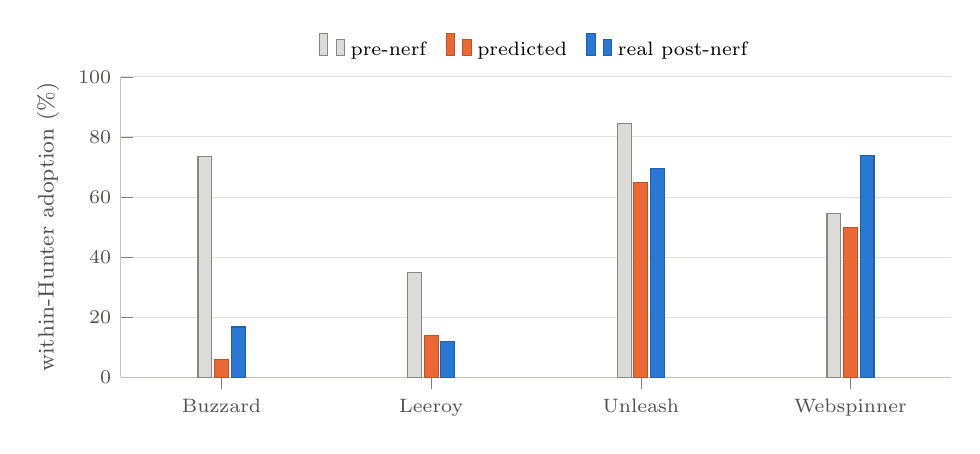
\begin{tikzpicture}
\begin{axis}[
  width=\columnwidth, height=5.4cm,
  ybar, bar width=5pt,
  ymin=0, ymax=100, ylabel={within-Hunter adoption (\%)},
  symbolic x coords={Buzzard, Leeroy, Unleash, Webspinner},
  xtick=data,
  enlarge x limits=0.16,
  axis line style={vizaxis},
  axis lines*=left,
  ymajorgrids, grid style={vizgrid},
  legend style={font=\scriptsize, at={(0.5,1.02)}, anchor=south,
                legend columns=3, draw=none,
                /tikz/every even column/.append style={column sep=5pt}},
  tick label style={font=\scriptsize, color=vizink},
  label style={font=\footnotesize, color=vizink}]
\addplot[bar shift=-6pt, draw=vizgray, fill=vizgray!30] coordinates
  {(Buzzard,73.4) (Leeroy,34.8) (Unleash,84.4) (Webspinner,54.4)};
\addlegendentry{pre-nerf}
\addplot[bar shift=0pt, draw=vizorange!80!black, fill=vizorange] coordinates
  {(Buzzard,6.1) (Leeroy,14.0) (Unleash,64.9) (Webspinner,50.0)};
\addlegendentry{predicted}
\addplot[bar shift=6pt, draw=vizblue!80!black, fill=vizblue] coordinates
  {(Buzzard,16.8) (Leeroy,12.0) (Unleash,69.5) (Webspinner,73.7)};
\addlegendentry{real post-nerf}
\end{axis}
\end{tikzpicture}
\caption{Hearthstone nerf-response prediction against reality
(three-seed ensemble). The nerfed pair falls to about where it really
landed; Unleash the Hounds is kept near its real rate, and Webspinner's
rise is missed. Gray gives the pre-nerf baseline, orange the model, blue
the real outcome.}
\label{fig:nerf}
\end{figure}

The no-change baseline ties the prediction on the overall adoption
Spearman after the expansion (0.71--0.77 against 0.72--0.78 by class)
and beats it after the nerf (0.88--0.92 against 0.71--0.74), for the
same reason it does in \pkmn{}: most cards do not move, and a baseline
that copies the roughly 100 unmoved cards is hard to beat on a rank
metric dominated by non-movers. The prediction's advantage is confined
to the movers, in direction and magnitude.

\subsection{Rolling-Trajectory Results}
\label{sec:hsrolling}

A rolling variant predicts the whole post-shock trajectory at the
archive's data resolution, five periods bounded by the two patch dates,
and separates two seeding regimes. In \emph{anchored} mode each period is
seeded from the previous period's real decks; in \emph{free-running} mode
only the first period is real and every later period starts from the
model's own previous elite population. Each mode runs at three seeds, ten
generations per period, and the reported trajectory is their mean.

Anchored one-step prediction holds up in every period: movers Spearman
runs 0.56--0.90 for every class and period (all $p\le0.03$), with
per-period level error of 2.4--4.0$\pp$. The predicted Buzzard trajectory
tracks the real collapse (Figure~\ref{fig:dissociation}), 73\%, 43\%,
11\%, and 6\% against a real 79\%, 53\%, 16\%, and 18\%, and Mad
Scientist and Webspinner sit within a few points of reality from the
second period on. The free-running forecast also reaches the collapse,
one period late (74\% where reality had fallen to 53\%, then 29\% and
3\%), and all three seeds drop the card by the final period. The cost of
free-running falls on the cards that rose. With no real decks re-entering
the loop, the evaluation gauntlet is drawn from the model's own
population, which never demands the new cards, and their adoption lags
reality by 20--45$\pp$ through the whole trajectory: Mad Scientist
reaches 34\% against 60\%, Webspinner 38\% against 68\%. Rank agreement
on movers falls to 0.30--0.67 after the first period and loses
significance for Mage after the nerf, and level error rises to
3.5--5.5$\pp$. Re-anchoring on real decks each period removes the lag.
The useful free-running horizon is one period, roughly six weeks; beyond
it the forecast keeps the direction of the shock and loses its levels.

\begin{figure}[t]
\centering
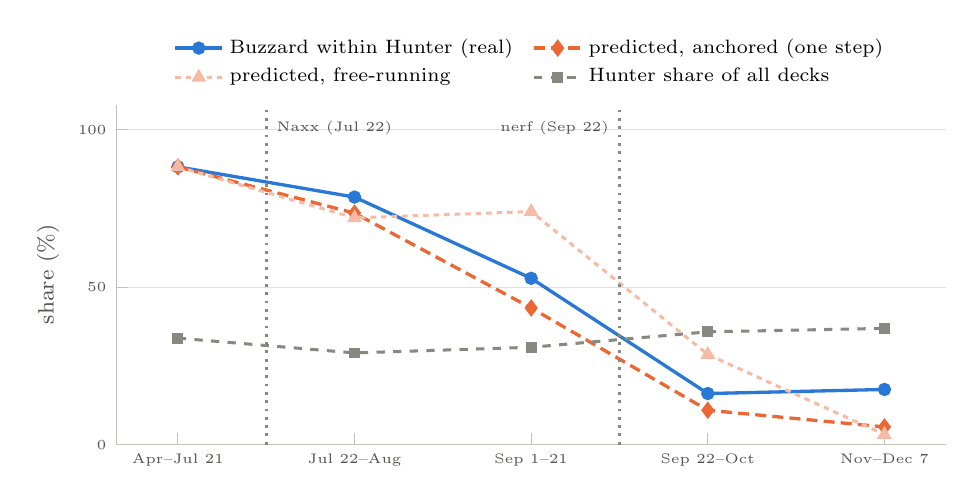
\begin{tikzpicture}
\begin{axis}[
  width=\columnwidth, height=5.9cm,
  ylabel={share (\%)},
  xmin=-0.35, xmax=4.35, ymin=0, ymax=108,
  xtick={0,1,2,3,4},
  xticklabels={{Apr--Jul 21},{Jul 22--Aug},{Sep 1--21},{Sep 22--Oct},{Nov--Dec 7}},
  axis line style={vizaxis},
  every tick/.style={vizaxis},
  ymajorgrids, grid style={vizgrid},
  axis lines*=left,
  legend style={font=\scriptsize, at={(0.5,1.02)}, anchor=south,
                legend columns=2, draw=none,
                /tikz/every even column/.append style={column sep=5pt}},
  legend cell align=left,
  tick label style={font=\tiny, color=vizink},
  label style={font=\footnotesize, color=vizink}]
\addplot[vizblue, line width=1.2pt, mark=*, mark size=1.8pt] coordinates
  {(0,88.2) (1,78.6) (2,52.8) (3,16.2) (4,17.5)};
\addlegendentry{Buzzard within Hunter (real)}
\addplot[vizorange, line width=1.2pt, dash pattern=on 4pt off 2.2pt,
         mark=diamond*, mark size=2.2pt, mark options={solid, fill=vizorange}]
  coordinates {(0,88.2) (1,73.5) (2,43.4) (3,10.9) (4,5.6)};
\addlegendentry{predicted, anchored (one step)}
\addplot[vizorange!45, line width=1.1pt, dash pattern=on 2pt off 1.8pt,
         mark=triangle*, mark size=2.0pt, mark options={solid, fill=vizorange!45}]
  coordinates {(0,88.2) (1,72.0) (2,74.0) (3,28.6) (4,3.2)};
\addlegendentry{predicted, free-running}
\addplot[vizgray, line width=1.1pt, dashed,
         mark=square*, mark size=1.4pt, mark options={solid, fill=vizgray}]
  coordinates {(0,33.8) (1,29.1) (2,30.9) (3,35.8) (4,36.9)};
\addlegendentry{Hunter share of all decks}
\draw[vizgray, dotted, line width=1pt] (axis cs:0.5,0) -- (axis cs:0.5,108)
  node[pos=0.93, right, font=\tiny, color=vizink] {Naxx (Jul 22)};
\draw[vizgray, dotted, line width=1pt] (axis cs:2.5,0) -- (axis cs:2.5,108)
  node[pos=0.93, left, font=\tiny, color=vizink] {nerf (Sep 22)};
\end{axis}
\end{tikzpicture}
\caption{The Hearthstone Buzzard trajectory at the archive's data
resolution, with both rolling modes (three-seed means). All model series
share the first point as input; everything after it is prediction.
Anchored, re-seeded from real decks, tracks the collapse; free-running,
re-seeded from its own population, reaches it one period late. Hunter's
class share (gray) never leaves its noise band.}
\label{fig:dissociation}
\end{figure}

\subsection{The Hidden-Information Ablation}
\label{sec:hsinfo}

Every result above uses agents that cannot see the opponent's hand.
Repeating the probe and the expansion-era evolution with agents trained
and run with both hands visible measures what hidden information
contributes. At the probe level the two protocols agree with each other
more than either agrees with the population. Per-class rank agreement
with real adoption is 0.35 against 0.34 for Hunter, 0.31 against 0.38
for Mage, and 0.59 against 0.61 for Warrior (hidden information first;
only the Warrior values are significant, $p<0.005$). Single cards move
more than the aggregates: Mad Scientist in Hunter probes at $+2.3\pp$
hidden against $+3.3\pp$ visible, and Duplicate at $-5.5\pp$ against
$-4.0\pp$.

At the evolution level, three seeds per protocol under the same
configuration, hidden information gives a lower pooled adoption error
(5.5 against 5.8$\pp$) and a higher mover direction rate (0.80 against
0.75), a modest aggregate gain. The card-level differences are larger.
With visible hands the pipeline over-adopts Mad Scientist (42.8\%
against a real 32.7\%, one seed at 76\%): an opponent who can see the
hand plays around nothing, so the card's body is pure tempo. It leaves
Death's Bite at 1.6\% (8.1\% under hidden information) and Webspinner at
13.4\% (33.9\%). Which cards evolution finds depends on the information
its pilots have, and the aggregate metrics understate the difference.

\section{Cross-Game Synthesis}
\label{sec:synthesis}

The two studies used different games, shocks, codebases, and ground truth. They agree on four findings, and on the evaluation practice the findings recommend.

\subsection{Composition versus Movement}
In both games the no-change baseline wins composition: \pkmn{} no-change
beats the framework on overlap in all four grid cells, and the
Hearthstone no-change baseline ties the pipeline on the overall adoption
rank correlation after the expansion and beats it after the nerf. In both, overlap sits near its ceiling because a metagame is
mostly stable across a shock, so it scores the fraction that did not move.
What each pipeline does predict is the movement: \pkmn{} edit-distance
delta beats no-change 42--0 at the high-ladder cutoff, and
Hearthstone probe-biased evolution predicts adoption direction and
magnitude on the cards that moved. A test a
do-nothing baseline can pass is measuring how stable the meta is, not how
good the method is. What is left, how much the meta moves and which way, is
where a real prediction shows itself, and both studies reach it
independently: one by replicating an existing framework, one by building a
new pipeline.

\subsection{Self-Referential Loops}
Each pipeline contains a place where the model's own output feeds its next
input, and in each, that loop degrades prediction. The \pkmn{} usage
refresh rebuilds teams from pickrates the builder itself wrote, and the
Hearthstone free-running forecast draws its evaluation gauntlet
from its own previous elite population. Neither has an outcome signal
that pulls it back toward what players did: \pkmn{} predictions worsen
when the refresh is faithful, and the Hearthstone forecast, evaluated
against opponents drawn from its own population, adopts the new cards at
about half their real rate and calls the nerf one period late. Both are
fixed the same way, by pulling the method back to real data at each step:
keeping the real month's statistics rather than the simulation's, or
re-seeding each period from real decks. That the same failure and the same fix appear in two
unrelated systems suggests the loop is a property of population-feedback
prediction itself, the same drift that population-based self-play has to
be designed around~\cite{lanctot2017unified,balduzzi2019openended}.

\subsection{Use of Simulated Outcomes}
In the tested ABC-Meta configuration, the team builder scores species by
their observed usage times their base stat total. Predicted usage comes
from counting appearances on the resulting teams. A species on a losing
team counts just as much as one on a winning team, so the forecast can be
computed without playing the battles. The battle-free rerun produces
almost unchanged predictions.

Hearthstone uses the games at two stages. The probe inserts a card into
fixed real decks and measures the change in win rate. Evolution proposes
cards with positive probe values more often, then plays the resulting
decks to decide which to retain. At the budgets tested, evolution without
the probe left new cards near the mutation floor. Selection still matters:
the probe favours keeping Leeroy, but its adoption falls during evolution
under the patched rules.

Our \pkmn{} surrogate is trained on simulated battle outcomes. During
search, it estimates a candidate team's win probability against reference
teams sampled from real usage, replacing fresh battles for each
comparison. Counting species in the teams found by search produces too
much change, so the final forecast blends the model's output with the
previous month's usage. Replacing that output with random noise and
applying the same blend does not reproduce the result. This control
supports a contribution from the learned model, although it does not
establish reliable predictions of which individual species will rise or
fall.

\subsection{Direction Prediction}
Neither study can say which particular unit will rise or fall. In \pkmn{},
the framework calls mover direction right about half the time ($0.53$), and the small
positive rank correlations it does show survive a control that carries no
real information about the change: shuffle a ranking and watch it drift back
toward the middle, and you get correlations of the same size for nothing.
In Hearthstone the probe's rank agreement with real adoption reaches
significance only for Warrior; at 22 cards per class, Hunter and Mage
stay below 0.4 under either information protocol. Calling the direction of specific movement is the problem this pair of
studies leaves open.

\subsection{Evaluation Recommendations}
Both studies argue for the same evaluation practice. Monthly \pkmn{} usage
transitions and period-resolved Hearthstone adoption both supply
many objective test cases on a fixed schedule, where hand-curated ban
scenarios cap evaluation at a handful. In both, a no-change baseline is
mandatory, paired significance tests should accompany point estimates, and
the reported metrics should be ones the baseline cannot trivially satisfy.
The \pkmn{} study adds the rating cutoff as a free parameter that flips the
headline comparison, and the Hearthstone study shows that how you read a predicted level off
the model matters as much as the model itself. Evaluating across regimes and cutoffs costs little; every boundary condition reported in this paper was found that way.

\section{Limitations}
\label{sec:limitations}

The \pkmn{} drift evaluation covers one tier of one generation; gen9ou is
the most played tier, but tier-specific dynamics could shift the numbers.
The exact-scenario rerun spans four tiers of Generation~8 only, with
fidelity notes on the reconstructions that current validators make
impossible. The 10{,}000-battle drift budget adds pickrate sampling noise
a larger budget would reduce, though Section~\ref{sec:battlefree} bounds
how much it can matter. The surrogate's strongest configuration carries a
post-hoc read-out-family caveat, partly answered by the cross-cutoff
transfer but not by a prospective test on future months. The rating-0 arm
ran the static configuration only.

The Hearthstone study uses three of the nine classes, so cross-class
effects are invisible to it. The probe swaps a card into fixed slots of
ordinary host decks, so cards whose value comes from a deck built around
them (Duplicate, Undertaker) are undervalued by design, and Death's Bite
is adopted well below its real rate at the 200-iteration search budget
used throughout. The one-shot predictions are three-seed ensembles with
the spread reported, but individual cards still swing across seeds. The
probe aggregates five hosts and 60 games per card but is itself a single
run. Across both studies, the ground-truth
archives are community-maintained and carry the collection biases of the
populations that produced them.

\section{Conclusion}

We asked what simulation predicts about a shifting metagame, and answered
it in two games with two independent pipelines. In \pkmn{} Showdown we
replicated a published meta discovery framework, reproduced its four ban
scenarios within one species, and mapped its operating envelope on a
completed grid of generations and rating cutoffs. In Hearthstone we
built a marginal-value probe and probe-biased evolution and predicted card
adoption across an expansion and a nerf against 33{,}697 real decklists.
The two agree. A no-change baseline wins the composition metric in both,
which saturates near its ceiling and measures stability rather than
prediction; what a simulator recovers is how much the metagame moves, on
the units that moved. Both pipelines contain a loop that feeds on their own output and degrades until grounded in real data, and in both the real starting usage carries the predictive content, with simulation only adding precision on top. The direction of specific movement remains unpredicted by every
method we tested. We contribute two methods aimed at the movement signal,
a fast learned stand-in for simulation, read out by blending toward no change, for \pkmn{} and a
marginal-value probe for Hearthstone, and a shared evaluation standard: a no-change baseline reported alongside every result, metrics that baseline cannot trivially satisfy, and more than one regime and cutoff.

\section*{Acknowledgments}

Claude models (Anthropic), primarily Claude Fable 5, were used throughout this work: as a coding assistant
for both experimental pipelines, to run and monitor the experiments, and
to draft and revise the manuscript under the authors' direction. The
authors reviewed all results and text and take full responsibility for
them.

\bibliographystyle{IEEEtran}
\bibliography{refs}

\end{document}
